The purpose of this case is to test the basic elements of an event based risk calculation, such as computation of the individual asset loss curves, the portfolio loss exceedance curve, average asset losses, and the average portfolio loss.

The list of assets and their taxonomies are shown in Table~\ref{tab:assets-tax1}, and Table~\ref{tab:vf-ln-tax1-zcov} shows the mean loss ratios and corresponding coefficients of variation in the vulnerability function used in this test case.

As in previous cases, ground motion fields are generated for each of the ruptures generated in the 100,000 stochastic event sets. These ground motion fields take into consideration both the inter-event and intra-event variability in the ground motion. The ground motion prediction equation used is Boore and Atkinson (2008), and the Jayaram and Baker (2009) model for spatial correlation of ground motion values is applied. These ground motion fields are also used for the corresponding calculation in Julia.

Since there is no variability in the loss ratio, calculation of the loss ratios is straightforward in this case. The loss tables for each of the seven assets in the portfolio is compiled in the same manner as described in the single asset Case~1a. Since the coefficients of variation in the vulnerability function are all zero, the lognormal distribution devolves into the degenerate distribution. Thus, the sampled loss ratio at a particular ground motion intensity level is always equal to the mean loss ratio at that intensity level obtained through interpolation. Since there is no random sampling of the loss ratios in this case, we should expect to find the results from OpenQuake and Julia to be exactly identical.

The portfolio loss curve calculated using the implementation of the calculator in Julia is compared with that produced by OpenQuake in Figure~\ref{fig:lc-ebr-6a}. Only the aggregated results for the portfolio are shown here for brevity.

\begin{figure}[htbp]
\centering
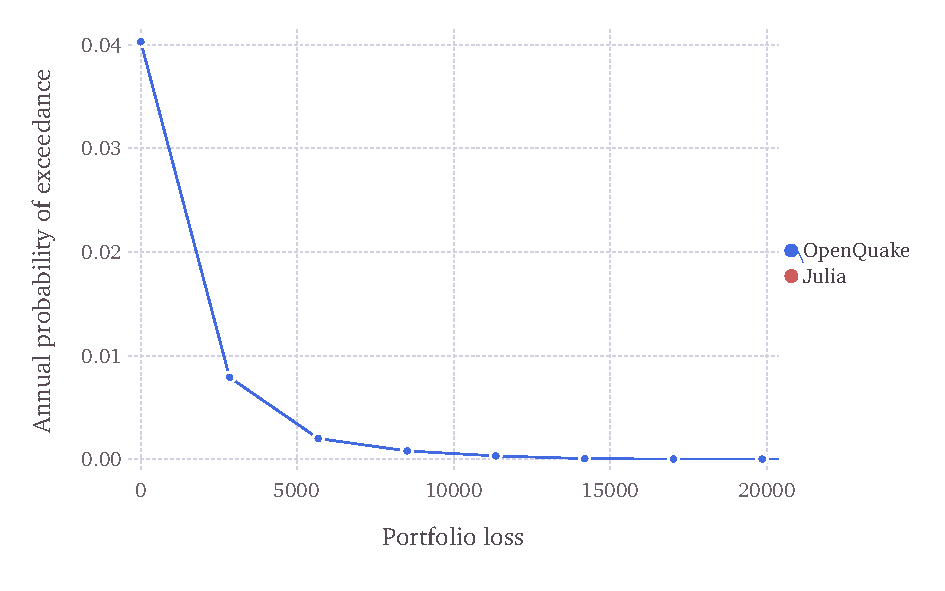
\includegraphics[width=12cm]{qareport/figures/fig-lc-ebr-6a}
\caption{Portfolio loss curve comparison for event based risk test case 6a}
\label{fig:lc-ebr-6a}
\end{figure}